\documentclass[aps,prb,twocolumn,groupedaddress,nofootinbib,floatfix]{revtex4}
%
\usepackage{graphicx} 
\usepackage{graphics}
\usepackage{epsfig}
\usepackage{caption}
\usepackage{amsmath}
\usepackage{bm}

%\setlength{\skip\footins}{0.3in}
\begin{document}
%
\title{Migration and Segregation in Three Dimensional Cellular Co-cultures: Role of
Differential Cell Adhesion and Elasticity}

%
\author{Daniel Kolbman}
%
% DON'T CHANGE ANYTHING IN THE NEXT FEW LINES OR DELETE BLANK LINES
%
\affiliation{This work was submitted as part of a course requirement for completion of the BS degree in the Physics Program at RIT and, in its current form, does not appear in any publication external to RIT.}
% % PUT YOUR ADVISOR NAME BELOW.  DON'T DELETE ANY LINES
%
\altaffiliation [Rochester Institute of Technology, School of Physics and Astronomy, Faculty Advisor: ]{Moumita Das}

\date{\today}

\begin{abstract} \noindent The biophysics of cell co-cultures, i.e. a binary system of cell populations, is of great interest in many biological processes including formation of embryos, and tumor progression. 
During these processes, different types of cells with different physical properties are mixed with each other, with important consequences for cell-cell interaction, aggregation, and migration. 
Until recently, experiments and theoretical models of cell co-cultures have focused on two dimensional systems. Under physiological conditions, however, cells often have to  
navigate three dimensional and confined micro environments. We will model such cell co-culture systems by extending previous $2D$ Brownian Dynamics simulation of a binary system of interacting, 
active, and deformable particles to a confined three-dimensional system. Our results will be compared with ongoing experiments done by our collaborators. Our results may 
provide insights into the role of the difference in physical properties such as cell elasticity, cell-cell adhesion, and cell self-propulsion speeds of two cell types in emergent collective properties 
such as cell aggregation and differential migration experimentally observed in co-cultures of breast cancer cells and healthy breast epithelial cells.  

\end{abstract}

\maketitle

\section*{Background and Motivation}

In several biological processes, from the formation of embryos to the formation and progression of tumors, cells with different physical properties are present in close proximity, with important
consequences for cell-cell interaction, aggregation, and migration. Laboratory cell co-cultures made of two different cell populations are ideal systems to qualitatively and quantitatively 
study how distinct physical properties of cells can influence such emergent behavior. Here we construct and study a simple proof of concept model of a cell co-culture in three dimensions 
and under confinement to test the hypothesis that differential physical properties of cells can drive segregation and preferential migration in co-cultures.   
The experimental system that motivates our work is a co-culture of breast cancer cells and non-cancerous breast epithelial cells. 
This system provides an excellent platform because of the characteristic differences between the two cell types \cite{Lee,mingming}. 
The nucleus and cytoplasm of breast cancer cells have been found to have relatively low elastic moduli compared to their non-cancerous counterparts \cite{Lee}. 
As a result, the cancer cells are much more deformable. Recent experiments suggest that this mechanical mismatch may play a key role in cancer cell migration through a healthy
cell population \cite{Lee}. 

Until recently, most experiments and models of cell co-cultures have focused on two dimensional systems, with limited application to physiological conditions\cite{Jong}.
Recently, new techniques for observing co-cultures in three dimensions have become available\citep{Alessandri}.  Accordingly, we seek to formulate a minimal
model of co-culture cell mechanics in three dimensions by extending previous two dimensional simulations of binary systems of deformable and active colloids\cite{Butcher}.
Together with our experimental collaborators Drs Wu and Ma at Cornell university we aim to characterize the role of difference in physical properties -- 
cell-cell adhesion, cell stiffness, and self-propulsion in  aggregation and migration in co-cultures of breast cancer cells and non-cancerous cells in $3D$.
Furthermore, we will focus on confined systems to better recreate the physiological and experimental systems we are studying.
From a physics perspective, we will study the interplay of cell mechanics, and statistical mechanical in cell migration in a confined binary system in $3D$.
The main ingredients of the model are discussed below.\\


{\bf 1. Co-culture Systems: mechanical stiffness, cell-cell adhesion, and self-propulsion of cancer cells vs healthy cells}\\
The system we seek to model is a co-culture of breast cancer cells and non-cancerous breast epithelial cells. 
In laboratory experiments, when introduced to a monolayer of healthy cells, cancer cells have been observed to have higher migration rates than when in a monolayer of other cancerous cells \cite{Lee}.
In addition to the difference in stiffness \cite{Lee}, the adhesion properties of cancer cells have also been found to be drastically different from that of non-cancerous cells\cite{Jeanes}.
Most healthy cells adhere to each other via the protein E-cadherin when they come in contact. Cancer cells lack this adhesiveness. Cancer cells further show enhanced self-propulsion (i.e. how fast individual cells can propel themselves by consuming ATP or due to other internal forces in the absence of any other 
interaction forces), compared to non-cancerous cells of the same tissue type. The differences in the adhesiveness, stiffness, and self propulsion of the two cell types is a key ingredient in our model.\\
\\

{\bf 2. Cell migration in three dimensions--different from two-dimensional migration.}\\
Many experimental and theoretical studies have addressed various aspects of cell migration in two dimensions, including protrusion, adhesion, and retraction at the level of single cells, and collective motion at the multicellular level.
However, the {\it in vivo} environment for a crawling cell is typically a three-dimensional environment, consisting of the extracellular matrix (ECM) and surrounding cells.
Recent experiments show increased migration rates of cells in $3D$ matrices as opposed to  $2D$\cite{Cukierman}.

{\bf 3. Role of confinement}\\
Current experiments involve observing co-cultures inside of spherical capsules with diameters on the order of several hundred micro-meters and containing tens of cells\cite{Alessandri} (See FIG. \ref{fig:capsule}).
Given that confinement and finite system size can have important consequences for the statistical mechanics and collective properties of the cell-culture, it will be vital to account for them in our model.
The spherical capsules in the experiments we will model have an inner diameter of $50-700$ micro-meters and an outer diameter of $400-7000$ micro-meters.
The cells are present inside the inner capsule and have a dimensions of the order of $\sim 10$ micro-meters.
The region between the inner and outer diameters is occupied by a dense gel layer that the cells can not penetrate.
The outside of this layer is coated such that cells will not adhere to this layer. \\

\begin{figure}
  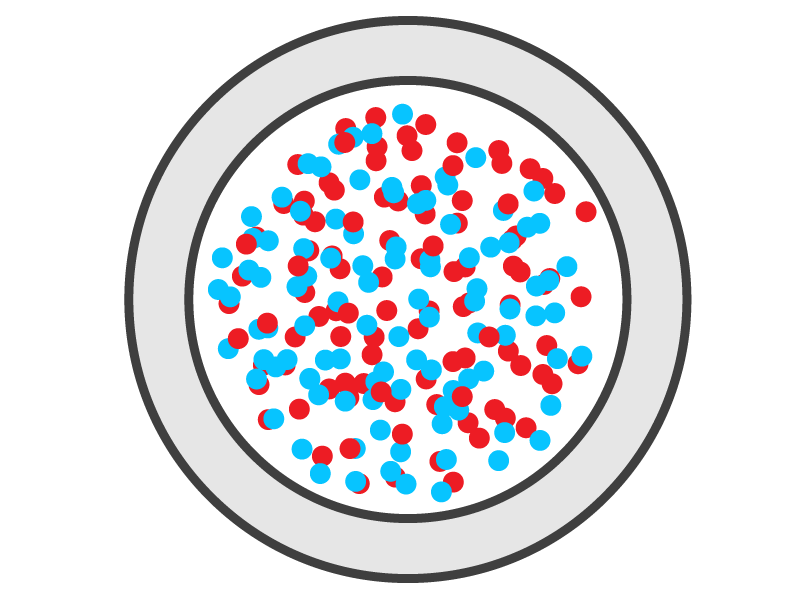
\includegraphics[width=3in]{Fig1.png}
  \caption[capsule]
   {A cross section of a spherical capsule enclosing a binary mixture of 
   cells.}
   \label{fig:capsule}
\end{figure}

{\bf 4. Interaction with the extra cellular matrix}\\
The ECM is a structural network of fibers that interact with the contained 
cells \cite{Alberts}. Healthy cells adhere to the ECM and move along it in
a manner mimicking $1D$ motion. Migration of cells in this manner has been 
observed to be significantly higher than in two dimensional matrices
\cite{Doyle}. Considering the ECM and its properties will thus be very 
important in the development of our three-dimensional model. 


\section*{Model}

We study the collective dynamics of this system using an active Brownian Dynamics simulation. Brownian dynamics is ideal for this system as cells behave like Brownian particles: 
their dimensions and times scale of motion are much larger than that of the particles of the surrounding medium in which they are suspended and in equilibrium  their motion is diffusive. In addition
our system is ``active" because cells can generate forces by consuming ATP and propel themselves. A simple model of homogeneous monolayers of such active particles consists
of a 2D system of interacting colloidal particles that are also each active, i.e. self-driven \cite{FilyMarchetti,RednerBaskaran}. 
Such models have been previously used to study swarming  behavior \cite{Vicsek} in birds, inspections and fish. Our group has recently combined this approach with cell 
mechanics and applied it to a binary population of cells, to study the collective mechanics and dynamics in cell co-cultures characterized by a difference in cell stiffness.
This study found that mechanical mismatch in co-cultures can have important consequences cell migration, and can lead to enhanced motility for more deformable cells\cite{Butcher}, 
in agreement with the Lee and coworkers \cite{Lee}. In this project, we extend this model to a three-dimensional system, include cell-cell adhesion, and further add the presence of a 
confining sphere to mimic the experimental set-up used by our collaborators \cite{mingming}. 


Our model co-culture is made of two sets A and B of active Brownian particles representing the cells (See FIG. \ref{fig:capsule}). The cells only interact with each other when 
they come into contact. The contact interaction between cells is of two types. First, when cells come into
contact and push against each other, depending on their mechanical stiffness they will respond with different forces; this interaction is modeled as an 
elastic repulsive interaction. For the non-cancerous (stiff) cells, there further exists a cell-cell adhesion,
modeled here as an attractive interaction at contact. The cancer (comparatively soft) cells do not have this adhesion. As for non-contact forces, 
the cancer cells can generate large self-propulsion forces. The self-propulsion forces generated by non-cancerous cells are orders of magnitude smaller in comparison 
and are assumed to be zero in our model. The strengths of the interactions are tuned to mimic physiological
conditions, where we use a stiffness of 2 KPa for the stiff (healthy) cells and a diffusion
constant of $1.8 \mu m^2/min$ for both cell types. The cancer cells are assumed to be up to ten times softer than their non-cancerous counterparts. 
Cell density is chosen to ensure a nearly confluent system. The particle positions evolve according to the over damped 
Langevin equations \cite{Lemons,RednerBaskaran,FilyMarchetti,Butcher}: 

\begin{equation}
  \bm{\dot{r}} = \frac{1}{\gamma}\bm{F}_{int}(\bm{r}) + v_p\hat{\bm{v}}_i+\sqrt{2D}\eta^T
\end{equation}

\begin{equation}
  \dot{\theta}_i=\sqrt{2D_r}\eta^R_i
\end{equation}

Where $F_{int}$ is the interaction forces on the cell from adhesion and repulsion.
$\bm{r}_i$ and $\dot{\bm{r}}_i$ is the position and velocity of the i\textit{th} particle, respectively.
The constant $\gamma$ is the damping coefficient of the fluid used. It is related to the
diffusion constant, $D$, by $D=\frac{k_BT}{\gamma}$, where $k_B$ is the Boltzman constant and $T$ is temperature. $v_p$ is the magnitude of propulsion
and $\bm{\hat{v}}_i$ is the direction of propulsion, $\bm{\hat{v}}=(cos\theta_i, sin\theta_i)$.
The noise $\eta^T$ represents fluctuations in translational motion and account for collisions with smaller fluid particles, while
$\eta^R$ is the rotational noise to simulate fluctuations in the direction of travel from ATP use by cells. 
Both types of noise follow the fluctuation dissipation theorem:

\begin{equation}
\left\langle \eta(t)\eta(t')\right\rangle = 0 
\end{equation}
\begin{equation}
\left\langle \eta(t)\eta(t')\right\rangle = 2k_bT\gamma
\delta(t-t')
\end{equation}

% Dimension stuff %
Both cell types have the same diameter  $\sigma$.
We define $k_BT$ and $\sigma$ to be our units of energy and length and define 
unit time as $\tau = \frac{\sigma^2}{D}$. These units are respectively used to non-dimensionalize 
energy, length, and time scales in the simulation. 

% Interaction forces %

The interaction forces are important for investigating how the elasticity and adhesivity of cells affects their migration and segregation. For non-cancerous cells, 
we have modeled the stiffness of the cells using a simple Hookean spring force while we use a `V' well to model the adhesion (See FIG. \ref{fig:interaction}). 
The result is particles that will desire to be close together, while resisting overlap. Cancer cells have the same qualitatively elastic repulsion, but not the cell-cell 
adhesion. For two cells whose centers are separated by a distance $r$, the repulsive and adhesive forces take the forms:

\begin{equation}
  F_{rep}(r) = F^0_{rep} \left\{ 
    \begin{array}{lr}
      1-\frac{r}{\sigma} &, r < 0\\
      0 &, r \ge \sigma
    \end{array}
  \right.
  \label{eq:frep}
\end{equation}

\begin{equation}
  F_{adh}(r) =F^0_{adh} \left\{
    \begin{array}{lr}
      0 &, r \le \sigma \\
      |r - (\sigma+\epsilon)|/\epsilon-1 &, \sigma < r < \sigma+2\epsilon
    \end{array}
  \right.
  \label{eq:fadh}
\end{equation}

The amplitudes of the interaction forces are chosen depending on the species of the particle. We denote these as $F^0_{rep}$ and $F^0_{adh}$ for the repulsive and adhesive prefactors, respectively.
The parameter $\epsilon$ is the phenomenological lengthscale over which the non-cancerous cells show cell-cell adhesion. 

\begin{figure}
  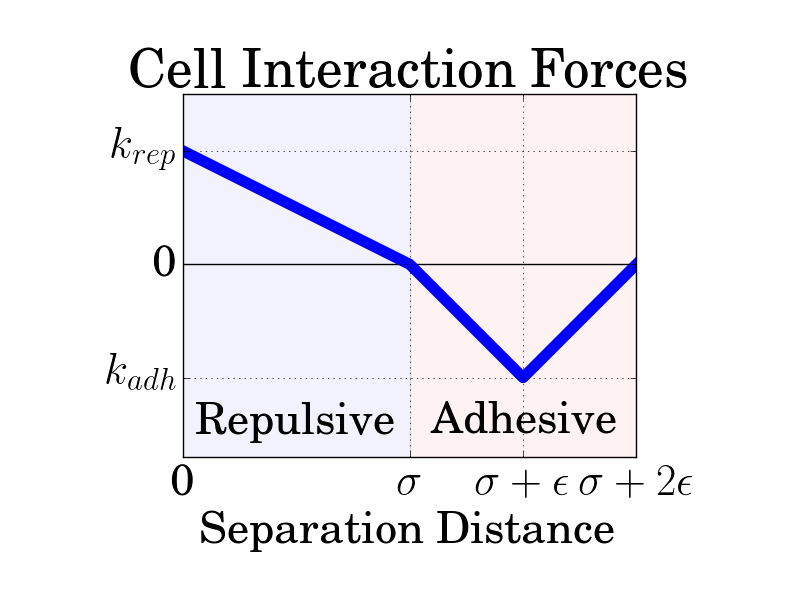
\includegraphics[width=1.0\columnwidth]{interaction.png}
  \caption[capsuleECM]{The two part interaction potential. For small separations
    within the diameter of the cells, there is a hookean, repulsive force. Separations
    outside, but near the cell, experience an adhesive force.}
   \label{fig:interaction}
\end{figure}

% Physical system (Boundaries, packing fraction) %

\subsection*{System Conditions}
We have imposed `hard' barrier boundaries on the system to imitate the conditions
of confining microfluidic shells used in the experiments \cite{mingming}. This means that particles may move along or within a
specified radius, but are restricted from moving outside of it. 
The size of the system is dependent on the packing fraction of the system. 
For our simulations, we choose a packing fraction of $\phi=0.4$, which is where 
active colloidal systems have been studied in the past\cite{RednerBaskaran}.
See FIG. \ref{fig:3dconf} for a sample 3D system.

\begin{figure}
  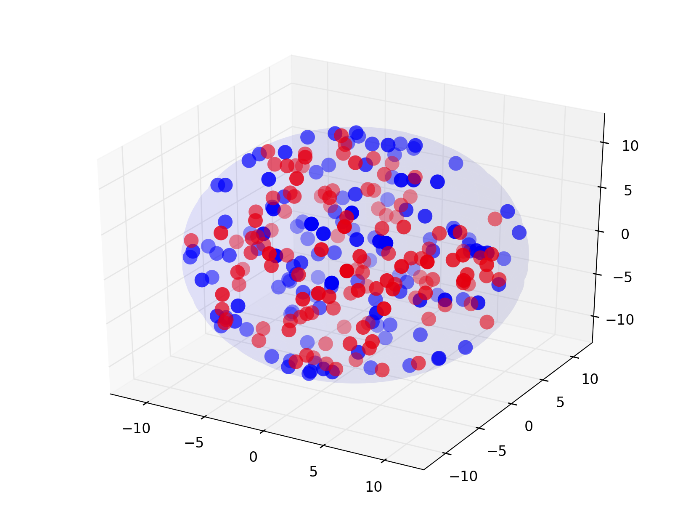
\includegraphics[width=1.0\columnwidth]{3dconf.png}
  \caption[3dconf]
    {A sample configuration of a 3D co-culture system.}
   \label{fig:3dconf}
\end{figure}

% Technical stuff %
\subsection*{Numerical Methods}

The dynamics simulations are computed in Julia, a high-performance, dynamic 
programming language for scientific computing. Spatial cell hashing and neighbor 
checking was used for broad phase collision detection to linearize run times 
as a function of the number of total particles. The simulations use a foreward 
Euler method to integrate with a time step of $10^{-6}\tau$. 
Many identical runs for each  simulation were run repeatedly in parallel and 
averaged together to produce data for a given set of parameters.

\section*{Preliminary Results}

Experimentally, when cancerous cells are immersed in populations of healthy cells
inside a microfluidic drop, the system experiences seperation behavior.The healthy 
cells will group in the the center of drop while the cancerous cells will collect
at the boundary. We are able to replicate this using our model.



\begin{widetext}
\begin{figure*}
  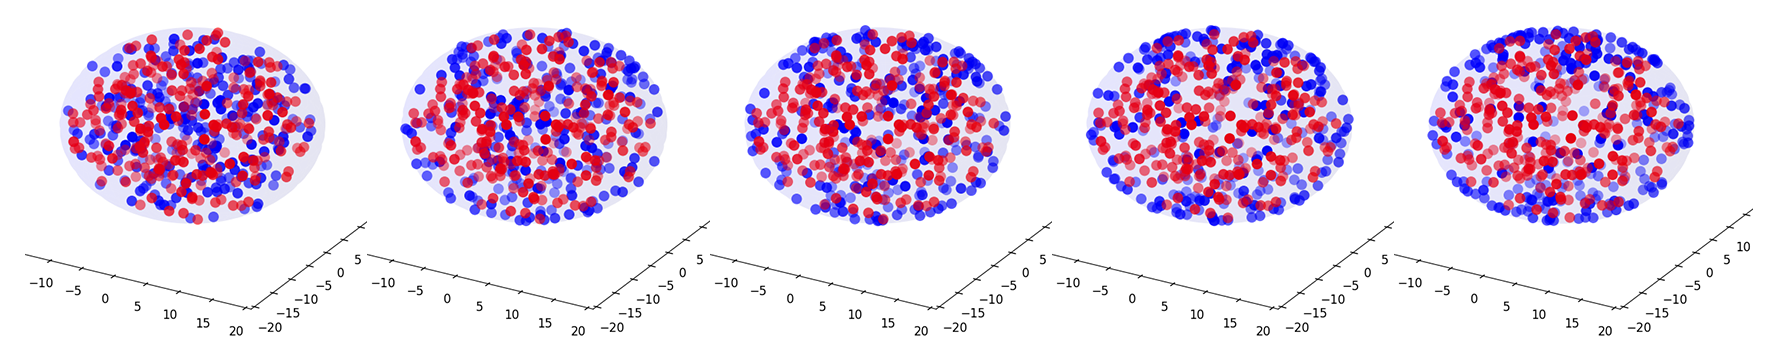
\includegraphics[width=\textwidth]{separation.png}
  \caption[separation]
    {Cancerous cells (Blue) separating over time (left to right)when immersed in healthy cells (Red)}
   \label{fig:separation}
\end{figure*}
\end{widetext}

\section*{Future Goals}

We have constructed a basic model to simulate the mechanics of a co-culture system. During the next semester, we plan to work closely with experimental data under physical parameters. We will focus on adding a few more components to our model that may be important to the roles of segregation and migration and what is being observed in the laboratory.
We will add an ECM (See FIG. \ref{fig:capsuleECM}), an important aspect that is present in the microcapsules, as a disordered potential.
The additional consideration of mitosis is another facet that may be important to the behavior of segregation. The division of cells may be important to the overall action of the system, particularly at the time scales that these effects are measured at. The difference in the rate of division between cancerous and healthy cells will also be an important aspect of mitosis and its contribution to the co-culture system.

\begin{figure}
  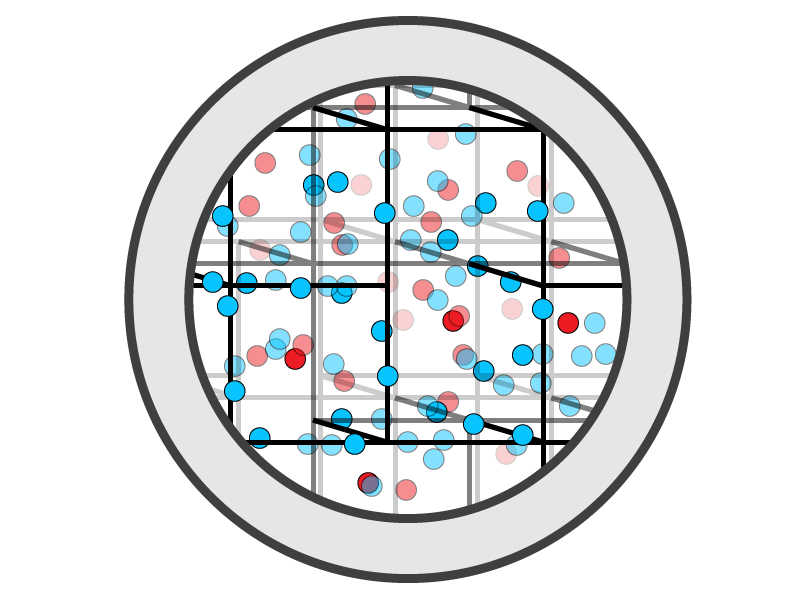
\includegraphics[width=1.0\columnwidth]{Fig2.png}
  \caption[capsuleECM]
   {A cross section of a spherical capsule enclosing a binary mixture of 
   cells and an extracellular matrix.}
   \label{fig:capsuleECM}
\end{figure}

\section*{Capstone II Timeline}
\begin{itemize}\itemsep1pt \parskip0pt
\item Apply experimental values for the inputs to the model, identify physiologically relevant regimes of parameters
and compare results of model thus far with control experiments in collaboration with Drs. Wu and Ma at Cornell. (2 weeks) 
\item Add extra cellular matrix in the form of a disordered weakly attractive potential. (4 weeks) 
\item Add mitosis (2 weeks)
\item Obtain results and analyze and interpreted  data. (2 weeks)
\item Attend March Meeting and present results (1 week)
\item Calculate phase diagram of aggregation and migration speed in terms of differential 
cell stiff, cell-cell adhesion, cell-matrix adhesion using experimentally relevant parameters. (2 weeks)
 \item Compare final results with experiments  write paper, give talk. (2 weeks)
\end{itemize}

\begin{acknowledgments}
Greatest thanks to: Dr. Moumita Das for her mentorship and assistance, Julian Butcher for his work in soft active colloids, Drs. Minglin Ma and Mingming Wu for their anticipated collaboration and experimental results, and Dr. Linda Barton for her arranging of Capstone Preparation.
\end{acknowledgments}

\vspace{0.6in}
%
%change the name of the bibliography file to your own name
%make sure you have h-physrev5.bst file in the same directory as your tex file and bib file
%then compile using Latex-Bibtex-Latex-Latex sequence!
%

\bibliographystyle{h-physrev5.bst}
% now the actual bibliography file.   Note that it does not need the .bib extension in this line!
\bibliography{DanKolbmanBibliographyFile}
\end{document}

